\section{Adjoint equation and optimality system of the \mbox{control} problem}

In this section we will use the formal Langrange method to derive the adjoint equation and the optimality system, as shown in \cite{optimalControl}. We use a Lagrange multiplier $p$ without proving its existence---the proof is deferred to Section \ref{proof}. The state system for our optimal control problem is given by \eqref{eq:heat}, a linear parabolic partial differential equation.
% Trenger vi denne her også?
% \begin{align*}
%       \rho c_p \theta_t - \nabla \cdot (k \nabla \theta) &= 0 \quad &\text{in } \Omega \\
%       -k \frac{\partial \theta}{\partial \nu} &= u(t) (\theta - \theta_w) \quad &\text{on } % \Gamma_1, \\
%       -k \frac{\partial \theta}{\partial \nu} &= 0 \quad &\text{on } \Gamma_0, \\
%       \theta(x, 0) &= \theta_0 &
% \end{align*}
The domain $Q = \Omega \times (0,T)$, for the hot rolling of steel is shown in Figure \ref{fig:steel_slab}. The blue arrows represent the coolant being sprayed onto the steel slab. The boundary $\Gamma_1$ is drawn as a solid line, with the dashed lines representing $\Gamma_2$. 
\begin{figure}
    \centering
    % 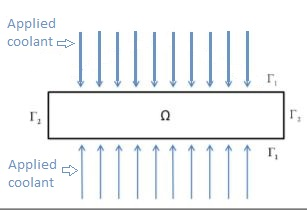
\includegraphics{figures/steel_slab_visualization.jpg}
    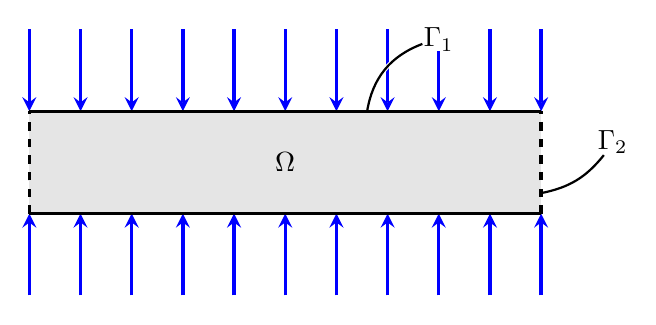
\begin{tikzpicture}[very thick, >=stealth, scale=1.3]
\draw (0, 0) -- (5, 0);
\draw (0, 1) -- (5, 1);
\draw[dashed] (0, 0) -- (0, 1);
\draw[dashed] (5, 0) -- (5, 1);
\node (domain) at (2.5, .5) {$\Omega$};
\foreach \x in {0, 0.5, ..., 5} {
    \draw[->, color=blue] (\x, -.8) -- (\x, 0);
    \draw[->, color=blue] (\x, 1.8) -- (\x, 1);
}
\node[fill=white, inner sep=0] (gamma1-1) at (4, 1.7) {$\Gamma_1$};
\node[fill=white, inner sep=0] (gamma2-1) at (5.7, 0.7) {$\Gamma_2$};
\draw[ultra thick, color=white] (gamma1-1) to [bend right=30] (3.3, 1);
\draw[thick] (gamma1-1) to [bend right=30] (3.3, 1);
\draw[thick] (gamma2-1) to [bend left=20] (5, 0.2);
\fill[black!10] (0, 0) rectangle (5, 1);
\draw (0, 0) -- (5, 0);
\draw (0, 1) -- (5, 1);
\draw[dashed] (0, 0) -- (0, 1);
\draw[dashed] (5, 0) -- (5, 1);
\node (domain) at (2.5, .5) {$\Omega$};
\end{tikzpicture}
    \caption{An illustration of our steel slab with applied cooling in blue, i.e. the control. The border $\Gamma_2$ is isolated in our modelling of the optimal control problem \eqref{eq:heat}.}
    \label{fig:steel_slab}
\end{figure}

More generally, one may consider a domain $\Omega \subset \mathbb{R}^3$ which is bounded with a Lipschitz boundary, $\partial \Omega = \Gamma_1 \cup \Gamma_2$. A suitable function space for the solution of a linear parabolic PDE is 
\begin{equation}
    \label{eq:funcSpace}
    W(0,T) : = \{ \theta \in L^2(0,T;H^1(\Omega)) : \quad \frac{\partial \theta}{\partial t} \in L^2(0,T;(H^1(\Omega))^{*}) \}
\end{equation}
We endow this space with the following norm, let $u \in W(0,T)$ then 
\begin{equation*}
    \|u\|_{W(0,T)} := \bigg (\int_{0}^T\|u(t)\|^2_{H^{1}(\Omega)}\dt \bigg ) ^{\frac{1}{2}} + \bigg (\int_{0}^T\|u'(t)\|^2_{H^{1}(\Omega)^{*}}\dt \bigg ) ^{\frac{1}{2}}
\end{equation*}
This is also a Hilbert space with the inner product given by 

\begin{equation*}
    \langle u, v \rangle_{W(0,T)} := \int_{0}^T\langle u(t),v(t) \rangle _{H^{1}(\Omega)}\dt  +  \int_{0}^T \langle u'(t), v'(t) \rangle_{H^{1}(\Omega)^{*}}\dt 
\end{equation*}

We follow the notion by \cite{optimalControl} and therefore the notation $L^{p}(a,b,X)$ means the linear space of all equivalence classes of measurable vector valued functions $u:[a,b] \rightarrow X$ which have the property that
\begin{equation*}
    \int_{a}^b\|u\|_X^p \dt<\infty.
\end{equation*}

We call a function vector-valued when it maps from $[a,b] \subset \mathbb{R}$ into a Banach space $X$. 

\subsection{The adjoint eqution and the gradient}
We start by finding the weak formulation for the problem defined in \eqref{eq:heat}. We multiply the equation \eqref{eq:heat-in-omega} by a test function $\psi\in H^{1,1}(Q)$, a function which has weak first-order partial derivatives in space and time. We then integrate over the domain $Q$. We assume that the heat conductivity, $k$, heat capacity $c_p$ and density $\rho$ are all constant, so that partial integration in space yields 
\begin{equation}
\begin{aligned}
  0 &= \iint_Q (\theta_t - \frac{k}{\rho c_p}\Delta\theta)\psi\dxdt  \\
  &= \iint_Q \theta_t\psi\dxdt + \frac{k}{\rho c_p}\iint_Q\nabla\theta \cdot \nabla\psi\dxdt - \frac{k}{\rho c_p}\iint_{\partial Q}\partial_\nu\theta\psi\dsdt.
\end{aligned}
\end{equation}
After using the boundary conditions defined in \eqref{eq:heat}, we end up with the following weak formulation of the state equation:
\begin{equation}\label{eq:weak-form}
  \begin{gathered}
  \iint_Q \theta_t\psi\dxdt + \frac{k}{\rho c_p}\iint_Q\nabla\theta \cdot \nabla\psi\dxdt + \frac{1}{\rho c_p}\iint_{\Sigma_1} u(t)(\theta - \theta_w)\psi\dsdt = 0,\\[1ex]
  \theta|_{t=0} = \theta_0,
  \end{gathered}
\end{equation}
where $\Sigma_i = \Gamma_i\times(0,T)$. We view $\theta_t$ as being in the space $ L^2(0,T;H^1(\Omega)^{*})$. Not that all terms pertaining to the boundary $\Sigma_2$ vanishes from the weak form, due to the assumption that no heat flows across this boundary. Now one can use a density argument to lessen the requirement on the test function such that we only require that $v \in W(0,T)$ which is introduced below. In fact this weak formulation is even valid for $v \in L^2(0,T,H^1(\Omega))$. 

From the weak formulation of the problem, we can easily set up the Lagrangian function, by subtracting the weak formulation of the problem \eqref{eq:weak-form} from the cost functional \eqref{eq:cost-func}. The test function is replaced with a Lagrange multiplier function $p$. This gives
\begin{equation}
  \begin{aligned}\label{eq:lagrangian-raw}
  \L(\theta, u, p) = &\,J(\theta, u) - \iint_Q \theta_t p\dxdt - \frac{k}{\rho c_p}\iint_Q\nabla\theta \cdot \nabla p \dxdt \\
  &- \frac{1}{\rho c_p}\iint_{\Sigma_1} u(t)(\theta - \theta_w)p \dsdt
  \end{aligned}
\end{equation}
As we will see in Section 3, we have that our Lagrangian is a map from 
\begin{equation*}
    \L : W(0,T)\cap C(\bar{Q}) \times L^{\infty}(0,T) \times  W(0,T) \cap C(\bar{Q}) \rightarrow \mathbb{R}
\end{equation*}.

\subsubsection{Adjoint equation}
The adjoint equation is derived by setting the directional derivative of the Lagrangian with respect to the state variable equal to zero. Assume the direction $h\in H^1(Q)$ is such that $h(x, 0) = 0$. % Antagelsen h(x, 0) = 0 popper visst ut av seg selv hvis man gjør noe på en bestemt måte i følge Dietmar.
This gives
\begin{equation}
  \begin{aligned}
  0 = \L_\theta(\theta, u, p)h = \int_\Omega (\theta(x,T) - \theta_d)h(x, T)\dx - \iint_Q h_t p\dxdt \\
  - \frac{k}{\rho c_p}\iint_Q\nabla h\nabla p \dxdt
  - \frac{1}{\rho c_p}\iint_{\Sigma_1} u(t)h p\dsdt.
  \end{aligned}
\end{equation}
Partial integration in time and in space then yields
\begin{equation} % Skip this calculation?
  \begin{aligned}
  0 = \L_\theta(\theta, u, p)h = \int_\Omega \theta(x,T) - \theta_d)h(x, T)\dx - \int_\Omega hp\Big|_0^T \dx \\
  + \iint_Q h p_t\dxdt
  + \frac{k}{\rho c_p}\iint_Q h\Delta p \dxdt \\
  - \frac{k}{\rho c_p} \iint_{\partial Q}\partial_\nu p\cdot h\dsdt
  - \frac{1}{\rho c_p}\iint_{\Sigma_1} u(t)h p\dsdt.
  \end{aligned}
\end{equation}
After some reordering of the terms we get
\begin{equation}
  \begin{aligned}
  0 = \L_\theta(\theta, u, p)h = \int_\Omega \theta(x,T) - \theta_d-p(x, T))h(x, T)\dx \\
  + \iint_Q h \left( p_t + \frac{k}{\rho c_p}\Delta p\right) \dxdt
   - \frac{k}{\rho c_p} \iint_{\Sigma_0}\partial_\nu p\cdot h\dsdt \\
   - \frac{1}{\rho c_p} \iint_{\Sigma_1}h(  k\partial_\nu p + u(t)p )\dsdt.
  \end{aligned}
\end{equation}
Let $h\in H_0^1(Q)$, i.e. $h$ vanishes at the boundary. Then we are left with the second integral only, which must still equal zero for every $h$ in the chosen function space. We then get
\begin{equation*}
  \rho c_p p_t + k\Delta p = 0 \quad\textrm{ in } \Omega.
\end{equation*}
Letting $h\in H^1(Q)$ such that $h(x, T) = 0$ and $h|_{\Sigma_0}=0$ gives
\begin{equation*}
  -k\frac{\partial p}{\partial\nu} = u(t)p \quad\textrm{ in } \Sigma_1.
\end{equation*}
Replacing the last condition on $h$ from above with $h|_{\Sigma_1}=0$ yields
\begin{equation*}
  -k\frac{\partial p}{\partial\nu} = 0 \quad\textrm{ in } \Sigma_0.
\end{equation*}
Finally, let $h\in H^1(Q)$, and we find
\begin{equation*}
  p(x, T) = \theta(x, T) - \theta_d
\end{equation*}
This constitutes the \textit{adjoint equation}, which we restate below
\begin{subequations}\label{eq:adjoint-system}
   \begin{align} % Approved by Dietmar!
      \rho c_p p_t + k\Delta p &= 0 \quad\qquad\textrm{ in } \Omega \times (0,T) \label{eq:adjoint-system-eqn} \\
      {-k}\frac{\partial p}{\partial\nu} &= u(t)p \,\,\quad\textrm{ in } \Sigma_1 \label{eq:adjoint-system-bd-1} \\
      {-k}\frac{\partial p}{\partial\nu} &= 0 \,\quad\qquad\textrm{ in } \Sigma_0 \label{eq:adjoint-system-bd-2} \\
      \rho c_p p(x, T) &= \theta(x, T) - \theta_d. \quad \textrm{ in } \Omega
   \end{align}
   \label{eq:adjoint-eqn}
\end{subequations}
This adjoint equation for the adjoint state $p$ runs backwards in time, but since the final condition (i.e. $p(x,T)$) is prescribed instead of the initial condition, the problem is well-posed. If one had posed $p(x, 0)$ instead one would have gotten an ill-posed backward parabolic equation. The driving force is end-temperature difference between the desired state and the actual temperature state of the steel slab.

\subsubsection{Gradient}
With box constraints on the control (see equation\eqref{eq:box_constraints}) we can derive the variational inequality, a first-order necessary optimality condition to be satisfied by an optimal control $\bar{u} \in U_{ad}$. The variational inequality is given by 
\begin{equation*}
    \L_u(\bar{\theta},\bar{u},p)(u-\bar{u}) \geq 0\ \forall u\in U_{ad}
\end{equation*}
Let $h = u - \bar{u}$. We differentiate in direction $h$, but now note that $h\in H^1(0, T)$. This gives
\begin{equation}
\begin{aligned} % Fikk hjelp av Dietmar for denne, så den skal være good.
  \L_u(\theta, u, p) h &= \gamma\int_0^T uh \dt - \frac{1}{\rho c_p} \iint\limits_{0\,\,\Gamma_1}^{\,\,\,T}(\theta - \theta_w)ph \dsdt \\
  &= \int_0^T h \left( \gamma u - \frac{1}{\rho c_p} \int_{\Gamma_1}(\theta - \theta_w)p \mathop{ds} \right) \dt.
\end{aligned}
\end{equation}
Inserting the definition of $h$ yields the variational inequality for our system, which states that
\begin{equation}
    \label{eq:variational}
    \int_0^T (u - \bar{u})(t) \left( \gamma \bar{u} - \frac{1}{\rho c_p} \int_{\Gamma_1}(\bar{\theta} - \theta_w)p \mathop{ds} \right) \dt \geq 0\ \forall u \in U_{ad}
\end{equation}

The gradient of the reduced cost funtional $F(u) := J(y(u),u)$ can be obtained from 
\begin{equation*}
    F'(u) = \L_u(y(u),u,p(u))
\end{equation*}
%
The space $H^1(0,T)$ is a Hilbert space. By Riesz representation theorem we can identify $H$ with $H^{*}$ for any Hilbert space $H$. Therefore, by identifying an isomorphism % har vi funnet en isomorfisme?
we find that the $u$-derivative of the lagrangian and consequently the gradient of our reduced cost functional is
%
\begin{equation*}
    F'(u) = \L_u(\theta,u,p) = \gamma u - \frac{1}{\rho c_p}\int_{\Gamma_1}(\theta - \theta_w)p \ds.
\end{equation*}


\subsection{Optimality System}
The optimality system of our control problem \eqref{eq:heat} consists of the state equation, the adjoint equation, and the variational inequality. The two latter are obtained by requiring that the $y$- and $u$-derivative of the Lagrange function vanish, as we did above. The total optimality system is
%
\begin{align*}
    \begin{cases}
     \rho c_p \theta_t - \nabla \cdot (k \nabla \theta) = 0 \quad & \text{in $\Omega$}, \\
      -k \frac{\partial \theta}{\partial \nu} = u(t) (\theta - \theta_w) &\text{on } \Gamma_1, \\
      -k \frac{\partial \theta}{\partial \nu} = 0  &\text{on } \Gamma_0, \\
      \theta(x, 0) = \theta_0 
      \end{cases}
      \end{align*}
      \begin{align*}
      \begin{cases}
       \rho c_p p_t + k\Delta p &= 0 \quad\qquad\textrm{ in } \Omega \\
      -k\frac{\partial p}{\partial\nu} &= u(t)p \,\,\quad\textrm{ in } \Sigma_1 \\
      -k\frac{\partial p}{\partial\nu} &= 0 \,\quad\qquad\textrm{ in } \Sigma_2 \\
      \rho c_p p(x, T) &= \theta(x, T) - \theta_d.
      \end{cases}
      \end{align*}
\begin{equation*}
      \gamma u - \frac{1}{\rho c_p} \int_{\Gamma_1} (\theta - \theta_w)p \ds =0
\end{equation*}
%
This is a system of first order necessary optimality conditions. That is, if $\bar{u} \in U_{ad}$ is an optimal control to our optimal control problem and $\bar{\theta} = S(\bar{u})$ is the associated state, then there exists an adjoint state $\bar{p}$ such that the adjoint system is satisfied, and the variational inequality is satisfied. 


%Tror ikke vi trenger det under

\iffalse
Now one can restate this optimalilty system using the projection formula if one assume box-constraints. That is, if we assume
\begin{equation*}
    U_{\mathrm{ad}} := \{ u \in L^2(\Sigma_1): u_a(x,t) \leq u(x,t) \leq u_b(x,t) \text{ for a.e. } (x,t) \in \Sigma_1 \},
\end{equation*}
then a control $\bar{u} \in U_{\mathrm{ad}}$ and the associated state $\bar{\theta}$ is optimal if and only if it satisfy together with the adjoint state $p$ solving \eqref{eq:adjoint-eqn}  and $\gamma >0$ i.e. the regularisation parameter is positive that
\fi

%\begin{equation}
%    \label{eq:Proj_formula}
%    \bar{u}(x,t) = \mathbb{P}_{[u_a(x,t), u_b(x,t)]} \left\{\frac{1}{\gamma}\theta_w(x,t)p(x,t) \right\}
% \end{equation}